\documentclass[a4paper, 11pt]{article}

\usepackage[utf8]{inputenc}
\usepackage[T1]{fontenc}
\usepackage{graphicx, wrapfig}
\usepackage[top=3cm, bottom=3cm, left=3.2cm, right=3.2cm]{geometry}
\usepackage{lmodern}
\usepackage{fancyhdr}
\usepackage{color, colortbl}
\usepackage[usenames, dvipsnames]{xcolor}
\usepackage{amsmath}
\usepackage{amssymb}
\usepackage{mathrsfs}
\usepackage{amsthm}
\usepackage{pgf, pgfplots, tikz}
\usepackage{listings}
\usepackage{makeidx}
\usepackage{hyperref}
\usepackage{setspace}
\usetikzlibrary{calc}
\usetikzlibrary{plotmarks}
\usetikzlibrary{decorations.markings}
\usepackage{manfnt, multicol}
\usepackage[section]{algorithm}
\usepackage{algorithmicx, algpseudocode, listings}
% fixes a bug for closing parantheses
\usepackage{etoolbox}
\makeatletter
\patchcmd{\lsthk@SelectCharTable}{%
  \lst@ifbreaklines\lst@Def{`)}{\lst@breakProcessOther)}\fi}{}{}{}
\makeatother
\usepackage{array, multirow, longtable}
\usepackage{enumerate}
\usepackage[inline]{enumitem}
\usepackage[english]{babel}
\usepackage{caption, tabu}


%°°°°°°°°°°°°°°°°°°°°°°°°°°°°°°°°°°°°°°°°°°°°°°%
%----Définition de l'environnement listings----%
%°°°°°°°°°°°°°°°°°°°°°°°°°°°°°°°°°°°°°°°°°°°°°°%

\lstset{literate=
  {á}{{\'a}}1 {é}{{\'e}}1 {í}{{\'i}}1 {ó}{{\'o}}1 {ú}{{\'u}}1
  {Á}{{\'A}}1 {É}{{\'E}}1 {Í}{{\'I}}1 {Ó}{{\'O}}1 {Ú}{{\'U}}1
  {à}{{\`a}}1 {è}{{\`e}}1 {ì}{{\`i}}1 {ò}{{\`o}}1 {ù}{{\`u}}1
  {À}{{\`A}}1 {È}{{\'E}}1 {Ì}{{\`I}}1 {Ò}{{\`O}}1 {Ù}{{\`U}}1
  {ä}{{\"a}}1 {ë}{{\"e}}1 {ï}{{\"i}}1 {ö}{{\"o}}1 {ü}{{\"u}}1
  {Ä}{{\"A}}1 {Ë}{{\"E}}1 {Ï}{{\"I}}1 {Ö}{{\"O}}1 {Ü}{{\"U}}1
  {â}{{\^a}}1 {ê}{{\^e}}1 {î}{{\^i}}1 {ô}{{\^o}}1 {û}{{\^u}}1
  {Â}{{\^A}}1 {Ê}{{\^E}}1 {Î}{{\^I}}1 {Ô}{{\^O}}1 {Û}{{\^U}}1
  {œ}{{\oe}}1 {Œ}{{\OE}}1 {æ}{{\ae}}1 {Æ}{{\AE}}1 {ß}{{\ss}}1
  {ç}{{\c c}}1 {Ç}{{\c C}}1 {ø}{{\o}}1 {å}{{\r a}}1 {Å}{{\r A}}1
  {€}{{\EUR}}1 {£}{{\pounds}}1
}

\lstdefinestyle{luaCode}{
  basicstyle=\footnotesize,        	% the size of the fonts that are used for the code
  breakatwhitespace=true,         	% sets if automatic breaks should only happen at whitespace
  breaklines=true,                 	% sets automatic line breaking
  captionpos=t,                    	% sets the caption-position to bottom
  commentstyle=\footnotesize\ttfamily\color{Emerald},    	% comment style
  deletekeywords={...},            	% if you want to delete keywords from the given language
  escapeinside={¦}{¦)},         	% if you want to add LaTeX within your code
  extendedchars=true,              	% lets you use non-ASCII characters; for 8-bits encodings only, does not work with UTF-8
  rulecolor=\color{OliveGreen!80},
  frame=trbl,
  framexleftmargin=10.8pt,
  framexrightmargin=7.2pt,
  keepspaces=true,                 	% keeps spaces in text, useful for keeping indentation of code (possibly needs columns=flexible)
  keywordstyle=\small\bfseries\color{OliveGreen!80},   % keyword style
  language=[5.0]Lua,                 	% the language of the code
  morekeywords={job.position},            	% if you want to add more keywords to the set
  numbers=left,                    	% where to put the line-numbers; possible values are (none, left, right)
  numbersep=3pt,                   	% how far the line-numbers are from the code
  numberstyle=\tiny\color{Gray}, 	% the style that is used for the line-numbers
  resetmargins=false                    % sets margins to 0 in a list
  showspaces=false,                	% show spaces everywhere adding particular underscores; it overrides 'showstringspaces'
  showstringspaces=false,          	% underline spaces within strings only
  showtabs=false,                  	% show tabs within strings adding particular underscores
  stepnumber=2,                    	% the step between two line-numbers. If it's 1, each line will be numbered
  stringstyle=\color{RawSienna},     	% string literal style
  tabsize=2,                       	% sets default tabsize to 2 spaces
  title=\lstname,                   	% show the filename of files included with \lstinputlisting; also try caption instead of title
  xleftmargin=1cm,                      % sets left margin indentation
  xrightmargin=1cm                      % sets right margin indentation
}

\lstdefinestyle{gpCode}{
  basicstyle=\footnotesize,        	% the size of the fonts that are used for the code
  breakatwhitespace=true,         	% sets if automatic breaks should only happen at whitespace
  breaklines=true,                 	% sets automatic line breaking
  captionpos=t,                    	% sets the caption-position to bottom
  commentstyle=\footnotesize\ttfamily\color{Emerald},    	% comment style
  deletekeywords={...},            	% if you want to delete keywords from the given language
  escapeinside={¦}{¦)},         	% if you want to add LaTeX within your code
  extendedchars=true,              	% lets you use non-ASCII characters; for 8-bits encodings only, does not work with UTF-8
  rulecolor=\color{OliveGreen!80},
  frame=trbl,
  framexleftmargin=10.8pt,
  framexrightmargin=7.2pt,
  keepspaces=true,                 	% keeps spaces in text, useful for keeping indentation of code (possibly needs columns=flexible)
  keywordstyle=\small\bfseries\color{OliveGreen!80},   % keyword style
  language=Gnuplot,                 	% the language of the code
  morekeywords={linestyle},            	% if you want to add more keywords to the set
  numbers=left,                    	% where to put the line-numbers; possible values are (none, left, right)
  numbersep=3pt,                   	% how far the line-numbers are from the code
  numberstyle=\tiny\color{Gray}, 	% the style that is used for the line-numbers
  resetmargins=false                    % sets margins to 0 in a list
  showspaces=false,                	% show spaces everywhere adding particular underscores; it overrides 'showstringspaces'
  showstringspaces=false,          	% underline spaces within strings only
  showtabs=false,                  	% show tabs within strings adding particular underscores
  stepnumber=2,                    	% the step between two line-numbers. If it's 1, each line will be numbered
  stringstyle=\color{RawSienna},     	% string literal style
  tabsize=2,                       	% sets default tabsize to 2 spaces
  title=\lstname,                   	% show the filename of files included with \lstinputlisting; also try caption instead of title
  xleftmargin=1cm,                      % sets left margin indentation
  xrightmargin=1cm                      % sets right margin indentation
}


\newcommand{\N}{\mathbb{N}}
\newcommand{\Q}{\mathbb{Q}} 
\newcommand{\R}{\mathbb{R}}
\newcommand{\Z}{\mathbb{Z}} 
\newcommand{\C}{\mathbb{C}}
\renewcommand{\epsilon}{\varepsilon} 
\renewcommand{\phi}{\varphi}


\newcommand{\CodeBrackets}[1]{{\color{RoyalBlue}{#1}}}    % color of parantheses and brackets
\newcommand{\CodeDigits}[1]{{\color{RawSienna}{#1}}} % color of numbers

%change les légendes des listings
\DeclareCaptionFont{white}{\color{white}}
\DeclareCaptionFormat{listing}{%
  \centering
  {\colorbox{OliveGreen!80}{%
      \parbox{0.9\linewidth}{%
          \centering
          #1#2#3
        }
      }
    }
  }
\captionsetup[lstlisting]{%
  format=listing,
  labelfont=white,
  textfont=white, 
  singlelinecheck=false, 
  indention=0pt,
  margin=0pt, 
  font={bf,sf,small}
}


%%%%%%%%	Définitions des environnements de théorèmes	%%%%%%%%
%% style théorème, lemme, proposition
\theoremstyle{plain}


%% style définitions, exemples et remarques
\theoremstyle{definition}


% For syncronisation with skim
\synctex = 1



%\title{{\bfseries Large-Scale Distributed Systems}\\ {\Large Project 1: Gossip-based dissemination, Peer
%    Sampling System}}
\title{%
  \normalfont{\bfseries{\rule{\linewidth}{2pt} Large-Scale Distributed Systems\\Project 2: Distributed Hash Tables\\ %
    \vspace{-0.4cm}  \rule{\linewidth}{2pt}}}
  }
\author{Laurent \textsc{Hayez}}
% Remove command to get current date 
\date{\today}


\begin{document}



\renewcommand{\proofname}{{\scshape Proof}}
\renewcommand{\labelitemi}{\textbullet}


\maketitle

\renewcommand{\contentsname}{Table of contents}
%Table of contents
\tableofcontents



%%  Section 1: Introduction
\section{Introduction}
\label{sec:introduction}
  
  The main goal of this project is to implement Chord protocol in a basic way. Chord is a distributed lookup
  protocol that has a key-routing layer. The key-routing mechanism then permits to implement a distributed
  hash table on top of it. 

  We will start by implementing Chord with only successors and predecessors. This implementation is not
  optimal, as the search time is $O(n)$. But we can do much better by adding a finger table to each node,
  which will reduce the search time $O(\log n)$. This will be our next step.

  Finally, we will modifiy some functions in order to have a fault-tolerant implementation. That is the nodes
  can recover from other node's failure by updating periodically their successor and their finger table. We
  will analyze how nodes failures affect the system by looking at stale references in the finger tables, and
  we will also take a look at the search performance under churn.


%%  Section 2: The base Chord protocol

\section{The base Chord protocol}
\label{sec:base-chord-protocol}

  In this section, we will implement the base Chord protocol. At first, we will consider a simplified version
  of Chord with no finger table. Each peer will only have links to its successor and its predecessor, thus we
  expect the search time to be $O(n)$ hops, where $n$ is the number of peers in the ring. Secondly, we will add a
  finger table to each node so that the queries can be performed in $O(\log(n))$ hops. Finally we will compare
  both protocols' search efficiency for 500 queries per node.

  \subsection{Implementation without finger table}
  \label{sec:implementation-without-ft}
  
    As you can see in the file \texttt{Chord-v1-2.lua}, the only tricky function (at first sight at least) is
    \texttt{is\_between}. It works as follow (example for the bracket pair ``()''): as we have a ring topology, we
    must consider two cases, lower $<$ upper and upper $<$ lower. In the first case, nb $\in$ (lower, upper)
    if nb $>$ lower and nb $<$ upper. In the second case, we have that lower is the last element of the ring,
    and upper the first one (this can happen because we work modulo $2^m$). Thus nb $\in$ (lower, upper) if nb
    $>$ lower (that is between lower and $2^m$) or nb $<$ upper (that is between $0$ and upper). For the other
    bracket pairs, it is the same principle. This function will be used through the whole project.

    \texttt{Chord-v1-2.lua} implements both algorithms 1 and 2 provided in the instructions.


  \subsection{Implementation of the finger table}
  \label{impl-fing-table}

    \texttt{Chord-fingers-v1.lua} provides an implementation of the Chord protocol with a finger table. From
    the previous implementation, we changed the function \texttt{init\_neighbors} to three functions, namely
    \texttt{init\_finger\_table}, \texttt{update\_finger\_table} and \texttt{update\_others}. The function
    \texttt{join} was also changed to initialize the finger table when a node joins and to tell the other node
    in the ring to update their finger table. Finally, the function \texttt{find\_predecessor} was split into
    the function \texttt{closest\_preceding\_finger} and \texttt{find\_predecessor}. In view of task 3.4, we
    already implemented the hops' counter for the queries. As \texttt{successor = finger[1].node}, we deleted
    the variable \texttt{successor} and instead called the function \texttt{get\_successor}, which returns \texttt{finger[1].node}.

    The finger table is initalized as follow:
    
    \begin{center}
      \lstinputlisting[style=luaCode, caption=Initialization of the finger table for each node, label =
      listing:init-fing-table, firstline=51, lastline=55]{Chord-fingers-v1.lua}
    \end{center}

    Before joining the ring, the nodes know no other node, so all the fingers are initialized to nil. The
    start is where to start searching in the ring, this does not change so we initialize them to their correct
    value. Finally we simply set \texttt{finger[1].node} to \texttt{n}, that is the node itself is its own
    successor.


  \subsection{Search performances}
  \label{sec:search-performances}
  
    We start analyzing the search performance in the basic Chord implementation. We used a ring with 64 nodes
    and 500 queries per node. We randomly generated the 500 keys as follows:
    
    \lstinputlisting[style=luaCode, caption=Generating random keys, label =
      listing:gen-rand-keys, firstline=204, lastline=209]{Chord-v1-2.lua}

   
    In order to parse the produced logs, we used the following code in bash:
\begin{lstlisting}[style=luaCode, language=bash, caption=Parser for the logs]
grep "Number of hops:" Logs/log-task2-5-cluster.txt | sed -r 's/.*\t([0-9]{1,2})$/\1/g' | sort -n | uniq -c | sed -r 's/ +([0-9]+)/\2 \1/g' >> ParsedLogs/log-task2-5-cluster.txt
\end{lstlisting}
    
    We produced the plot shown in Figure \ref{fig:search-basic-chord}. We see that the we found approximately
    the same number of keys for each number of hops. This tells us, as we expected that the search time in the
    basic Chord is $O(n)$ where $n$ is the number of nodes in the ring. 


    \begin{figure}[h]
      \centering
      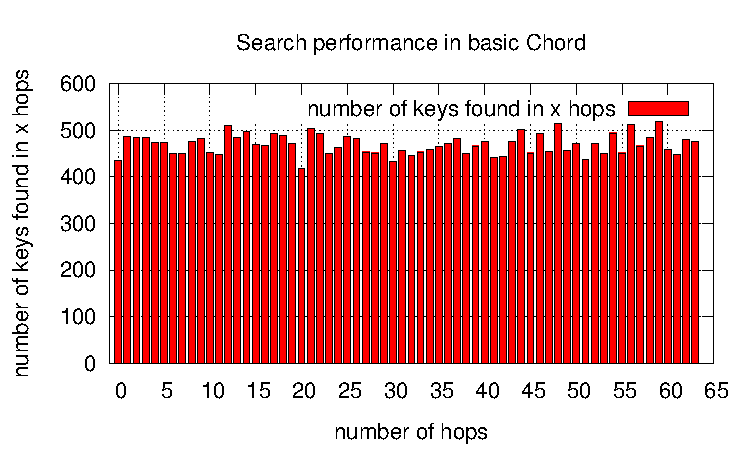
\includegraphics{plots/task2-2-cluster.pdf}
      \caption{Search performance in basic Chord}
      \label{fig:search-basic-chord}
    \end{figure}

    

    For the Chord implementation with a finger table, we used the same parameters and the same code to generate the keys. We
    obtained the results shown in Figure \ref{fig:search-perf-chord-fing-table}. As we expected, we can see
    that we obtain the keys in $O(\log(n))$ hops. To compare both plots, we put them together in Figure
    \ref{fig:comp-search-chord}. On this figure we clearly see how much the finger table helps to improve the
    search performance.

    \begin{figure}[h]
      \centering
      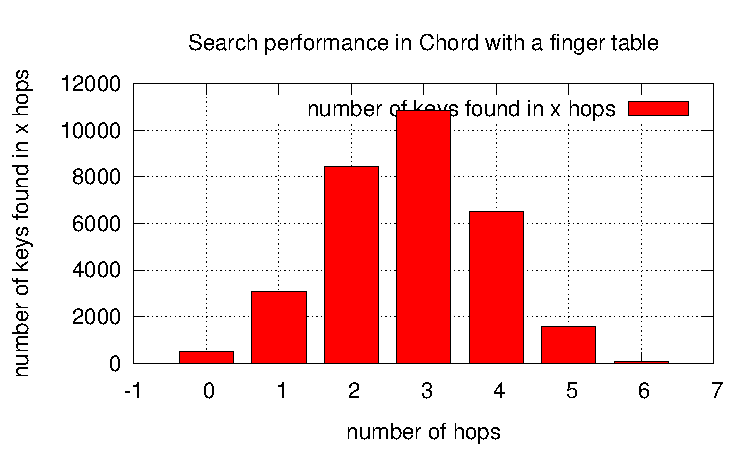
\includegraphics{plots/task2-5-cluster.pdf}
      \caption{Search performance in Chord with a finger table}
      \label{fig:search-perf-chord-fing-table}
    \end{figure}

    \begin{figure}[h]
      \centering
      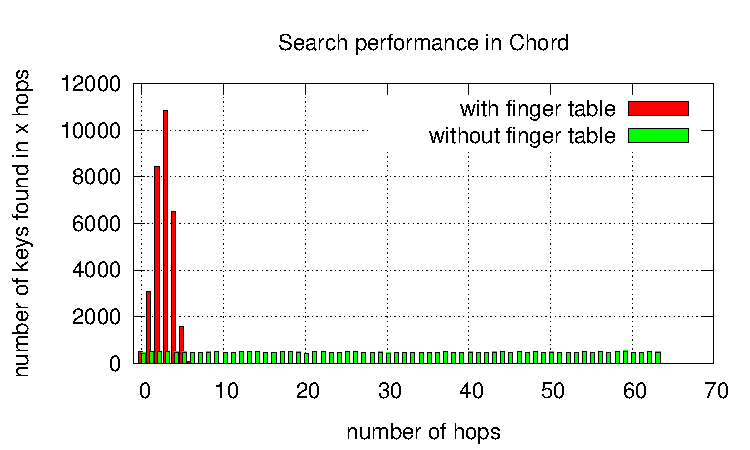
\includegraphics{plots/task2-5-cluster-compar.pdf}
      \caption{Comparison of the search performances in Chord}
      \label{fig:comp-search-chord}
    \end{figure}


\section{The Fault-Tolerant Chord Protocol}
\label{sec:fault-tolerant-chord}

  In the previous section, we assumed that once a node joined the ring, it would not leave it. In this section
  we present an implementation of Chord that can recover from nodes suddenly leaving the ring. We will analyze
  this implementation by looking at the stale references in the finger table. Finally we will evaluate the
  search performance under churn.

  \subsection{Implementation of the fault-tolerant Chord protocol}
  \label{sec:impl-ft-chord}
  
    We changed a little bit the join function from the given algorithm. We implemented it as follows:

    \lstinputlisting[style=luaCode, caption=join(n') for the fault-tolerant Chord protocol, label =
    listing:join, firstline=183, lastline=191]{Chord-fingers-v2.lua}

    The implementation of the fault-tolerant Chord protocol is provided in the file
    \texttt{Chord-fingers-v2.lua}. There is nothing tricky in this implementation, appart from the previously
    discussed parts. 
    
    
  \subsection{Analysis of the fault-tolerant Chord protocol}
  \label{sec:eval-ft-chord}

    We start analyzing the average number of stale references under churn. We consider a reference stale if it
    points to a node not available anymore, ie a non nil node not responding. To count the stale references,
    we used the following code:

    \lstinputlisting[style=luaCode, caption=Check for the stale references, label =
    listing:stale-refs, firstline=194, lastline=200]{Chord-fingers-v2.lua}

    The average number of stale references was calculated as
      \[\frac{\text{current number of stale
          references at current time}}{\text{total elapsed time}}.\]
    
    We made various plots, each with
    one different parameter varying. We used a set up of 64 nodes for the ring, and the provided churn trace
    to simulate the nodes leaving the ring. On Figure \ref{fig:Av-SR-fix-fingers}, we see that when we set the
    stabilization period to 10 seconds, the fix\_fingers period to 20 seconds and the check\_fingers period to
    20 seconds, we have less stale references than for the other periods. That result was surprising, so we
    launched the same experiment one more time, but as you can see the result was similar.

    We expected that the more we update the fingers, the less stale references we would obtain, but it is not
    what happens on Figure \ref{fig:Av-SR-fix-fingers}. When the fix\_finger period is 5 or 10 seconds, the
    results are quite similar, but surprisingly, when it is set to 20 seconds there are less stale
    references. For Figures \ref{fig:Av-SR-stab} and \ref{fig:Av-SR-check-finger}, we have approximately the
    same number of stale references, which is what we expected since we updated the fingers at the same
    frequency for all experiments

    \begin{figure}[h]
      \centering
      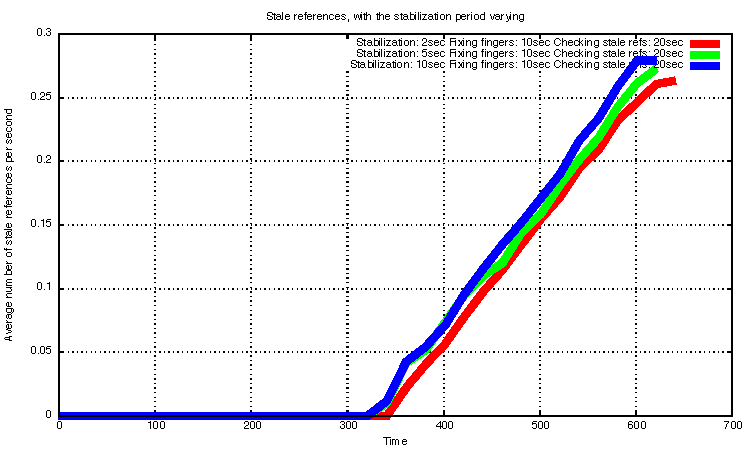
\includegraphics{plots/Average-SR-stabilization.pdf}
      \caption{Average number of stale references, with the stabilization period varying}
      \label{fig:Av-SR-stab}
    \end{figure}
    
    
    \begin{figure}[h]
      \centering
      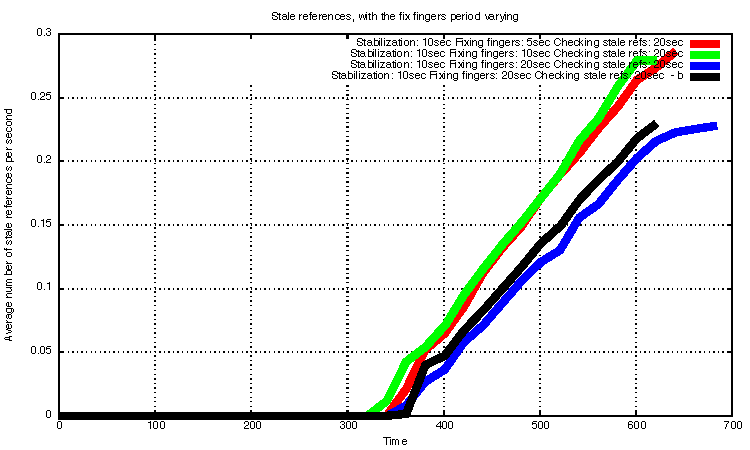
\includegraphics{plots/Average-SR-fix-fingers.pdf}
      \caption{Average number of stale references, with the fix\_fingers period varying}
      \label{fig:Av-SR-fix-fingers}
    \end{figure}
    
    
    \begin{figure}[h]
      \centering
      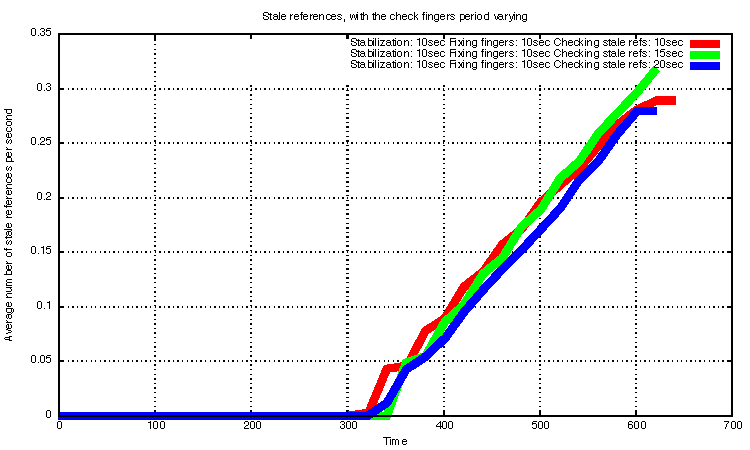
\includegraphics{plots/Average-SR-check-finger.pdf}
      \caption{Average number of stale references, with the check\_finger period varying}
      \label{fig:Av-SR-check-finger}
    \end{figure}

    

    We now analyze how the nodes recovers from churn. We can see on Figures \ref{fig:Rec-SR-stab},
    \ref{fig:Rec-SR-fix-fingers} and \ref{fig:Rec-SR-check-finger} that the finger table does not recover well
    from churn. This is due to the function \texttt{fix\_fingers}, shown in Listing \ref{listing:fix-fingers}. 

    \lstinputlisting[style=luaCode, caption=Function fix\_fingers, label =
    listing:fix-fingers, firstline=163, lastline=166]{Chord-fingers-v2.lua}

    This finger simply select a random finger and updates its reference, but the chosen finger might be a
    valid one and the stale entries will thus not be updated. And as this is done every 5, 10 or 20 seconds it
    would take a long time to remove all the stale entries of the finger table. A possible amelioration of
    this function could thus be to get the best of the functions \texttt{fix\_fingers} and
    \texttt{check\_fingers} to as shown in Listing \ref{listing:check-and-fix-fingers}.

    The results with this function are shown in Figures \ref{fig:Av-SR-fix-finger-am} and
    \ref{fig:Rec-SR-fix-finger-am}. The amelioration is not transcendent, but we see that we have
    approximately two times less stale references than before. \newpage

        \lstinputlisting[style=luaCode, caption=Function fix\_fingers ameliorated, label =
    listing:check-and-fix-fingers, firstline=163, lastline=169]{Chord-fingers-v2-amelioration.lua}


    We also see that, unlike before, this time the best result is obtained when we set the stabilization
    period to 10 seconds, the fix\_fingers period to 10 seconds and the check\_fingers period to 20 seconds. 

    \begin{figure}[h]
      \centering
      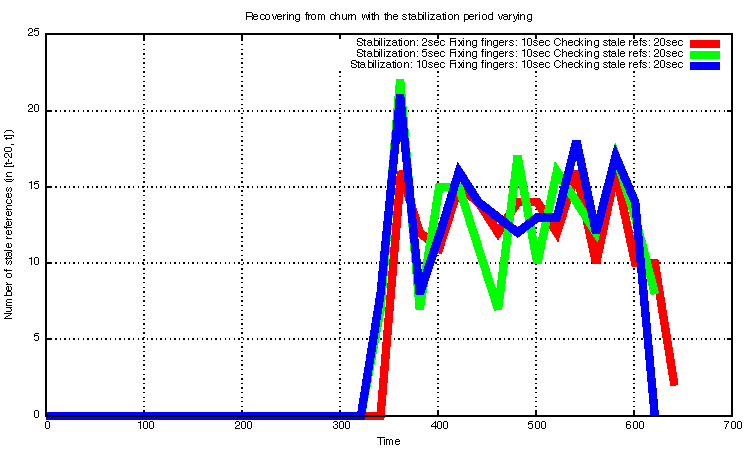
\includegraphics{plots/Recovery-SR-stabilization.pdf}
      \caption{Recovery of the finger table after churn, with the stabilization period varying}
      \label{fig:Rec-SR-stab}
    \end{figure}
    
    
    \begin{figure}[h]
      \centering
      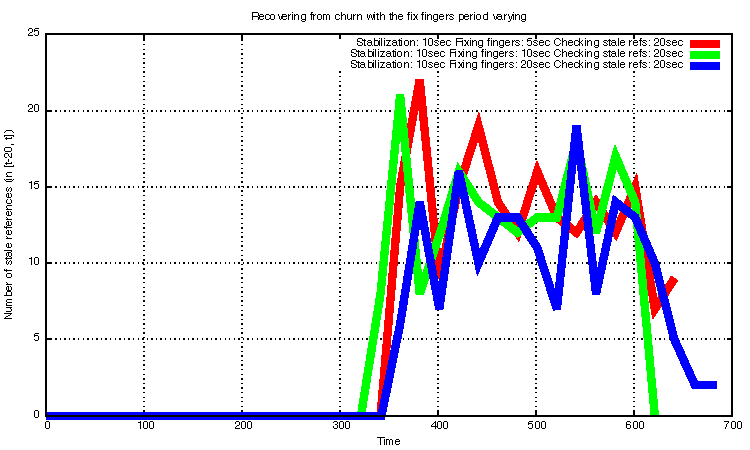
\includegraphics{plots/Recovery-SR-fix-fingers.pdf}
      \caption{Recovery of the finger table after churn, with the fix\_fingers period varying}
      \label{fig:Rec-SR-fix-fingers}
    \end{figure}
    
    
    \begin{figure}[h]
      \centering
      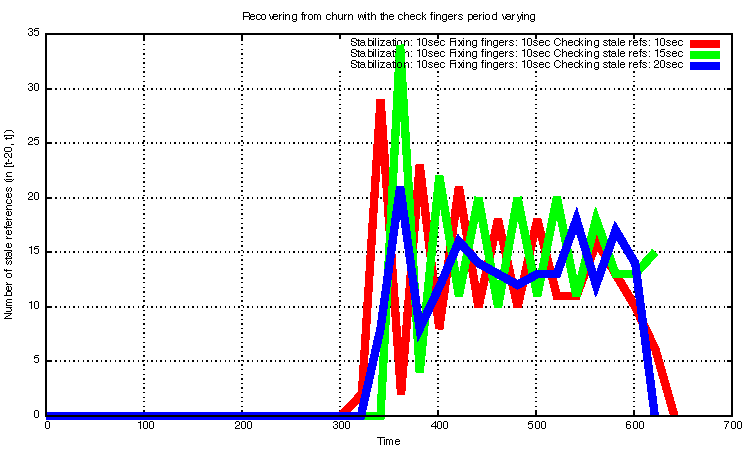
\includegraphics{plots/Recovery-SR-check-fingers.pdf}
      \caption{Recovery of the finger table after churn, with the check\_finger period varying}
      \label{fig:Rec-SR-check-finger}
    \end{figure}

    \begin{figure}[h]
      \centering
      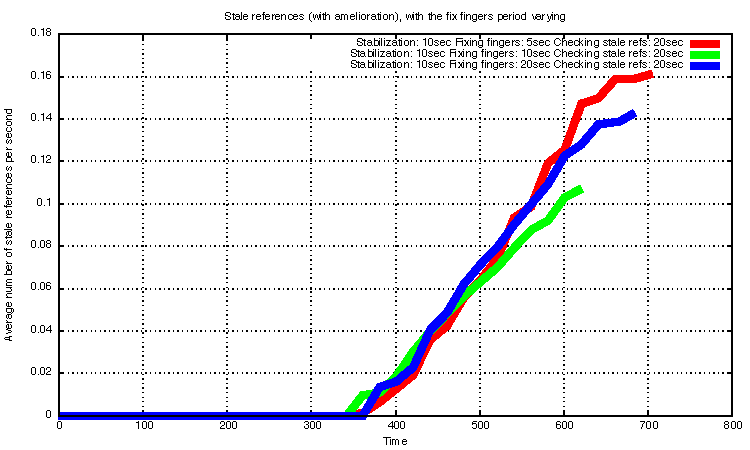
\includegraphics{plots/Average-SR-fix-fingers-ameliorated.pdf}
      \caption{Average number of stale references, with the ameliorated fix\_finger function}
      \label{fig:Av-SR-fix-finger-am}
    \end{figure}

    \begin{figure}[h]
      \centering
      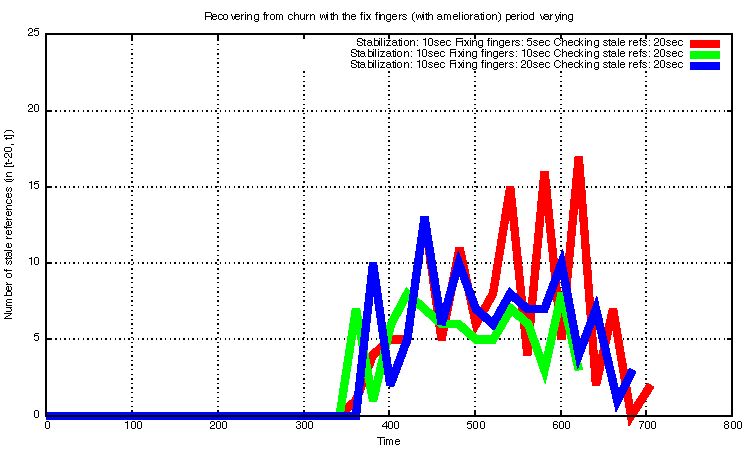
\includegraphics{plots/Rec-SR-fix-fingers-ameliorated.pdf}
      \caption{Recovery of the finger table after churn, with the fix\_finger (ameliorated) period varying}
      \label{fig:Rec-SR-fix-finger-am}
    \end{figure}
    

    \begin{figure}[h]
      \centering
      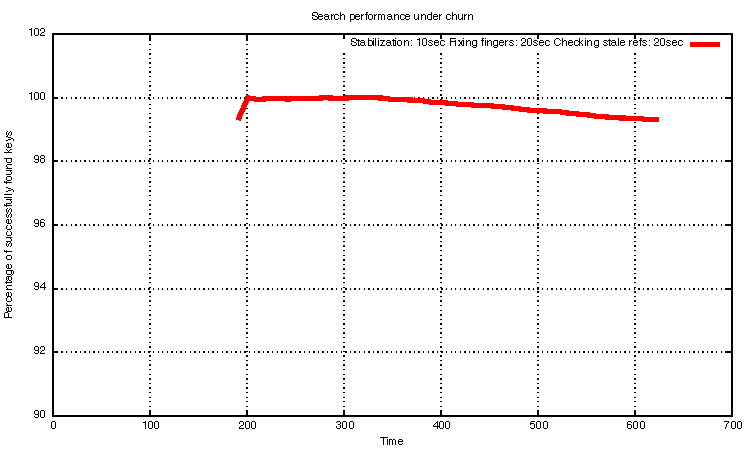
\includegraphics{plots/task3-5.pdf}
      \caption{Percentage of successfully found keys}
      \label{fig:percentage-successfully-found-keys}
    \end{figure}

    \begin{figure}[h]
      \centering
      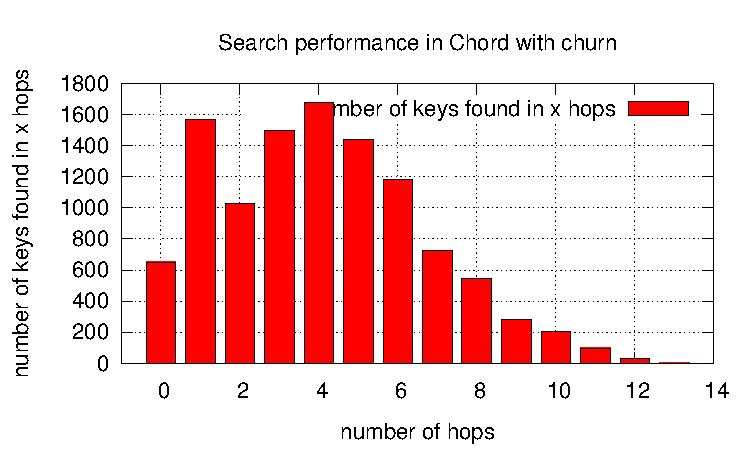
\includegraphics{plots/task3-5-cluster.pdf}
      \caption{Search performance in Chord with churn}
      \label{fig:search-perf-with-churn}
    \end{figure}



    
    
    












	
\end{document}



%%% Local Variables:
%%% mode: latex
%%% TeX-master: t 
%%% End: